\section{Frequency mode 19}
\label{FM19}
\subsection{Spectra}
\label{FM19:spectra}

\begin{figure}[ht]
    \centering
    \begin{subfigure}[b]{0.9545\textwidth}
        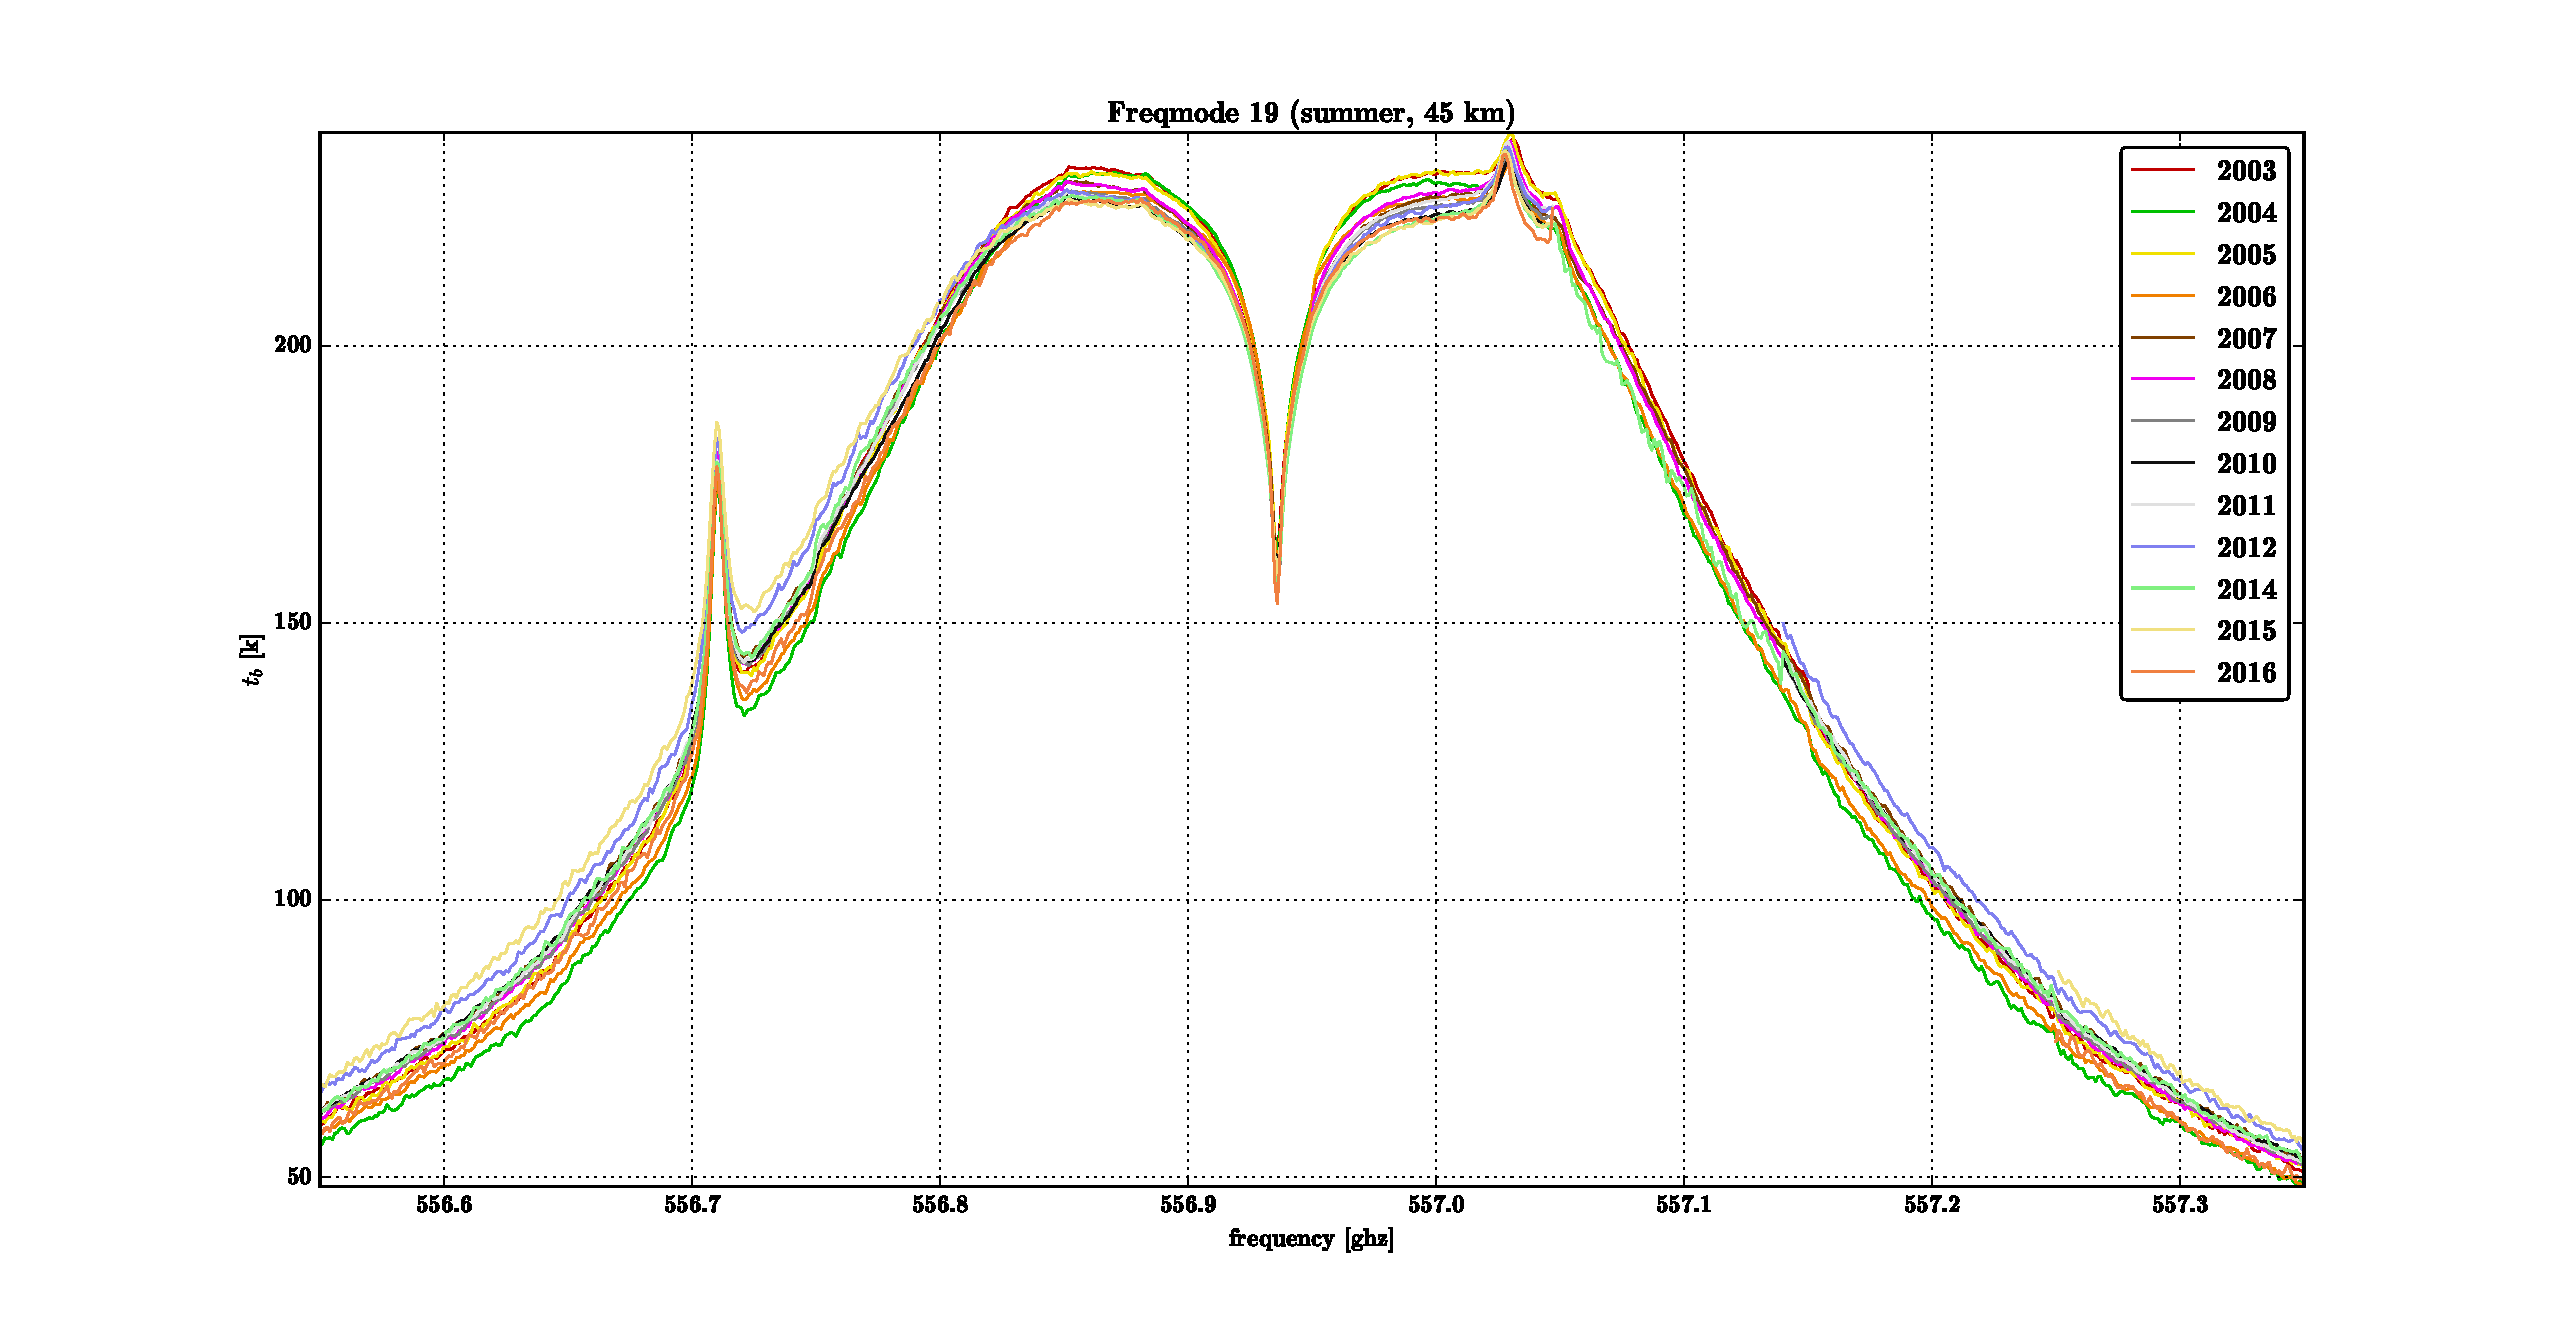
\includegraphics[width=\textwidth]{fm_19_spectra_summer_45km}
        \caption{summer; 2014--2016 from FM~119}\label{fig:spectra:19:summer}
    \end{subfigure}
    \begin{subfigure}[b]{0.9545\textwidth}
        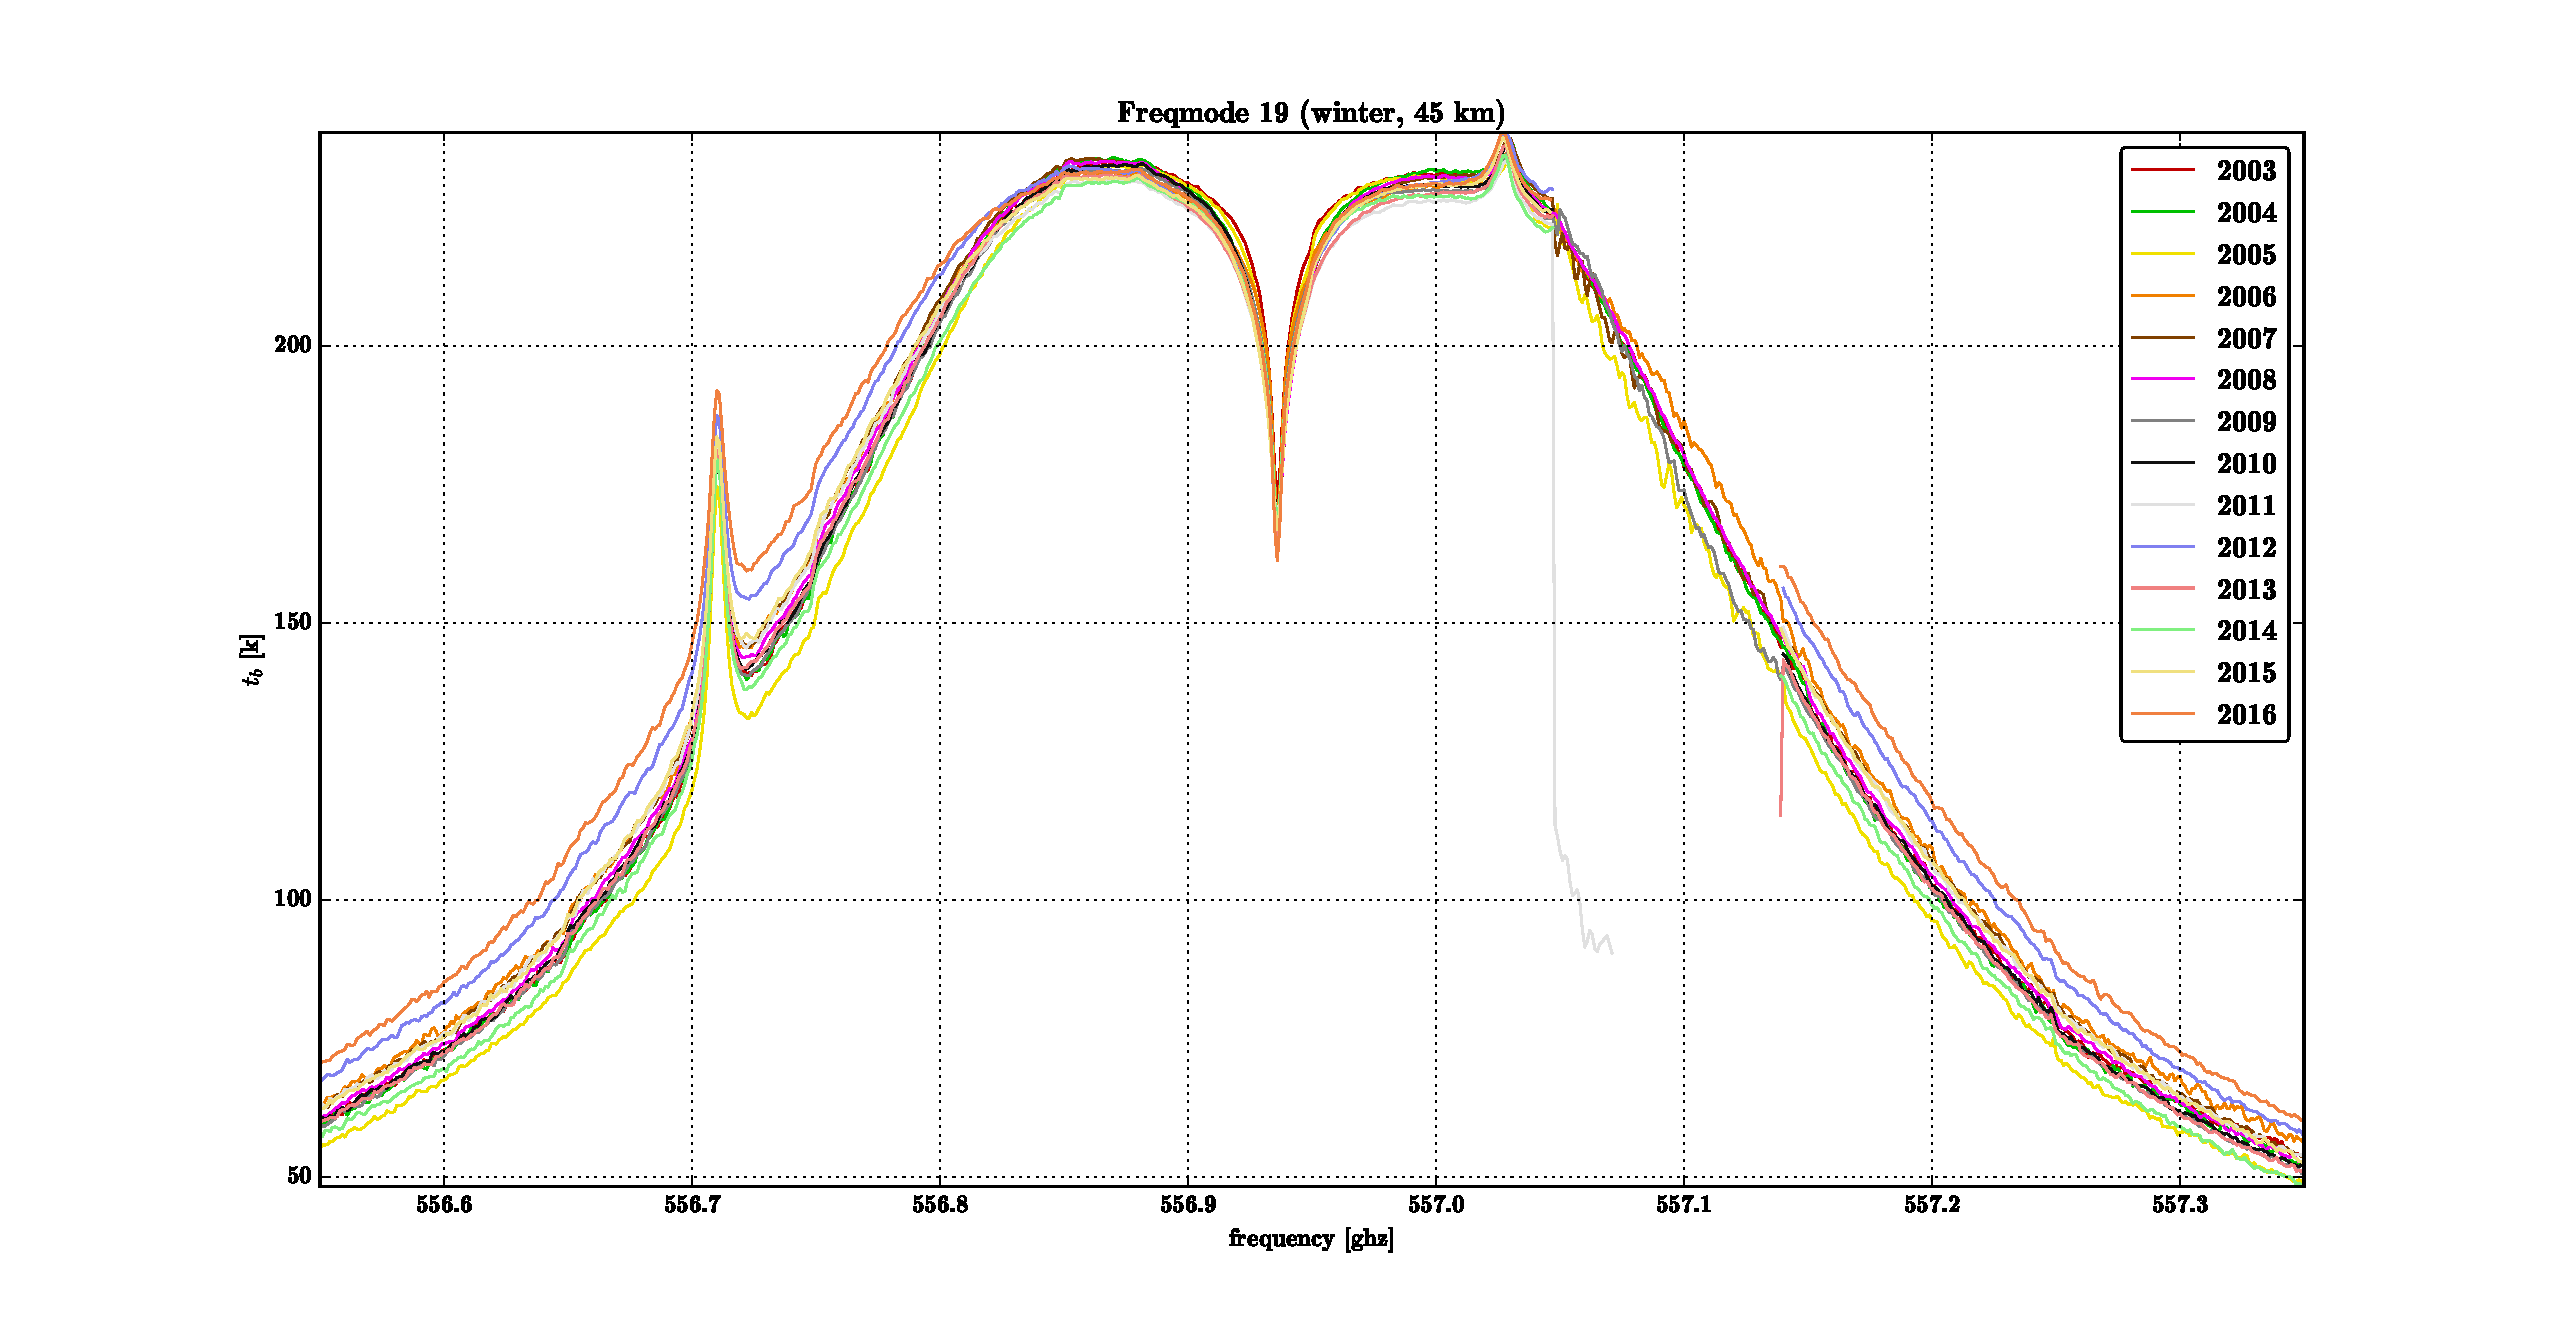
\includegraphics[width=\textwidth]{fm_19_spectra_winter_45km}
        \caption{winter}\label{fig:spectra:19:winter}
    \end{subfigure}
    \caption{Annual median spectra for FM~19 for altitude interval 42--48~km
        at equatorial latitudes.  The large ``double peak'' in the middle is
        \chem{H_2O}; peak on the left is \chem{O_3}; peak on the outer side of
        the right \chem{H_2O}-plateau is \chem{O_3} from sideband at
        $\sim541.071\,\mathrm{GHz}$.  The unhealthy sub-bands~2 and~1 encompass
        respectively: the whole of the right \chem{H_2O} peak (including the
        sideband peak); the following slope up to $\sim557.15\,\mathrm{GHz}$.
        }\label{fig:spectra:19}
\end{figure}

\begin{figure}[ht]
    \centering
    \begin{subfigure}[b]{0.9545\textwidth}
        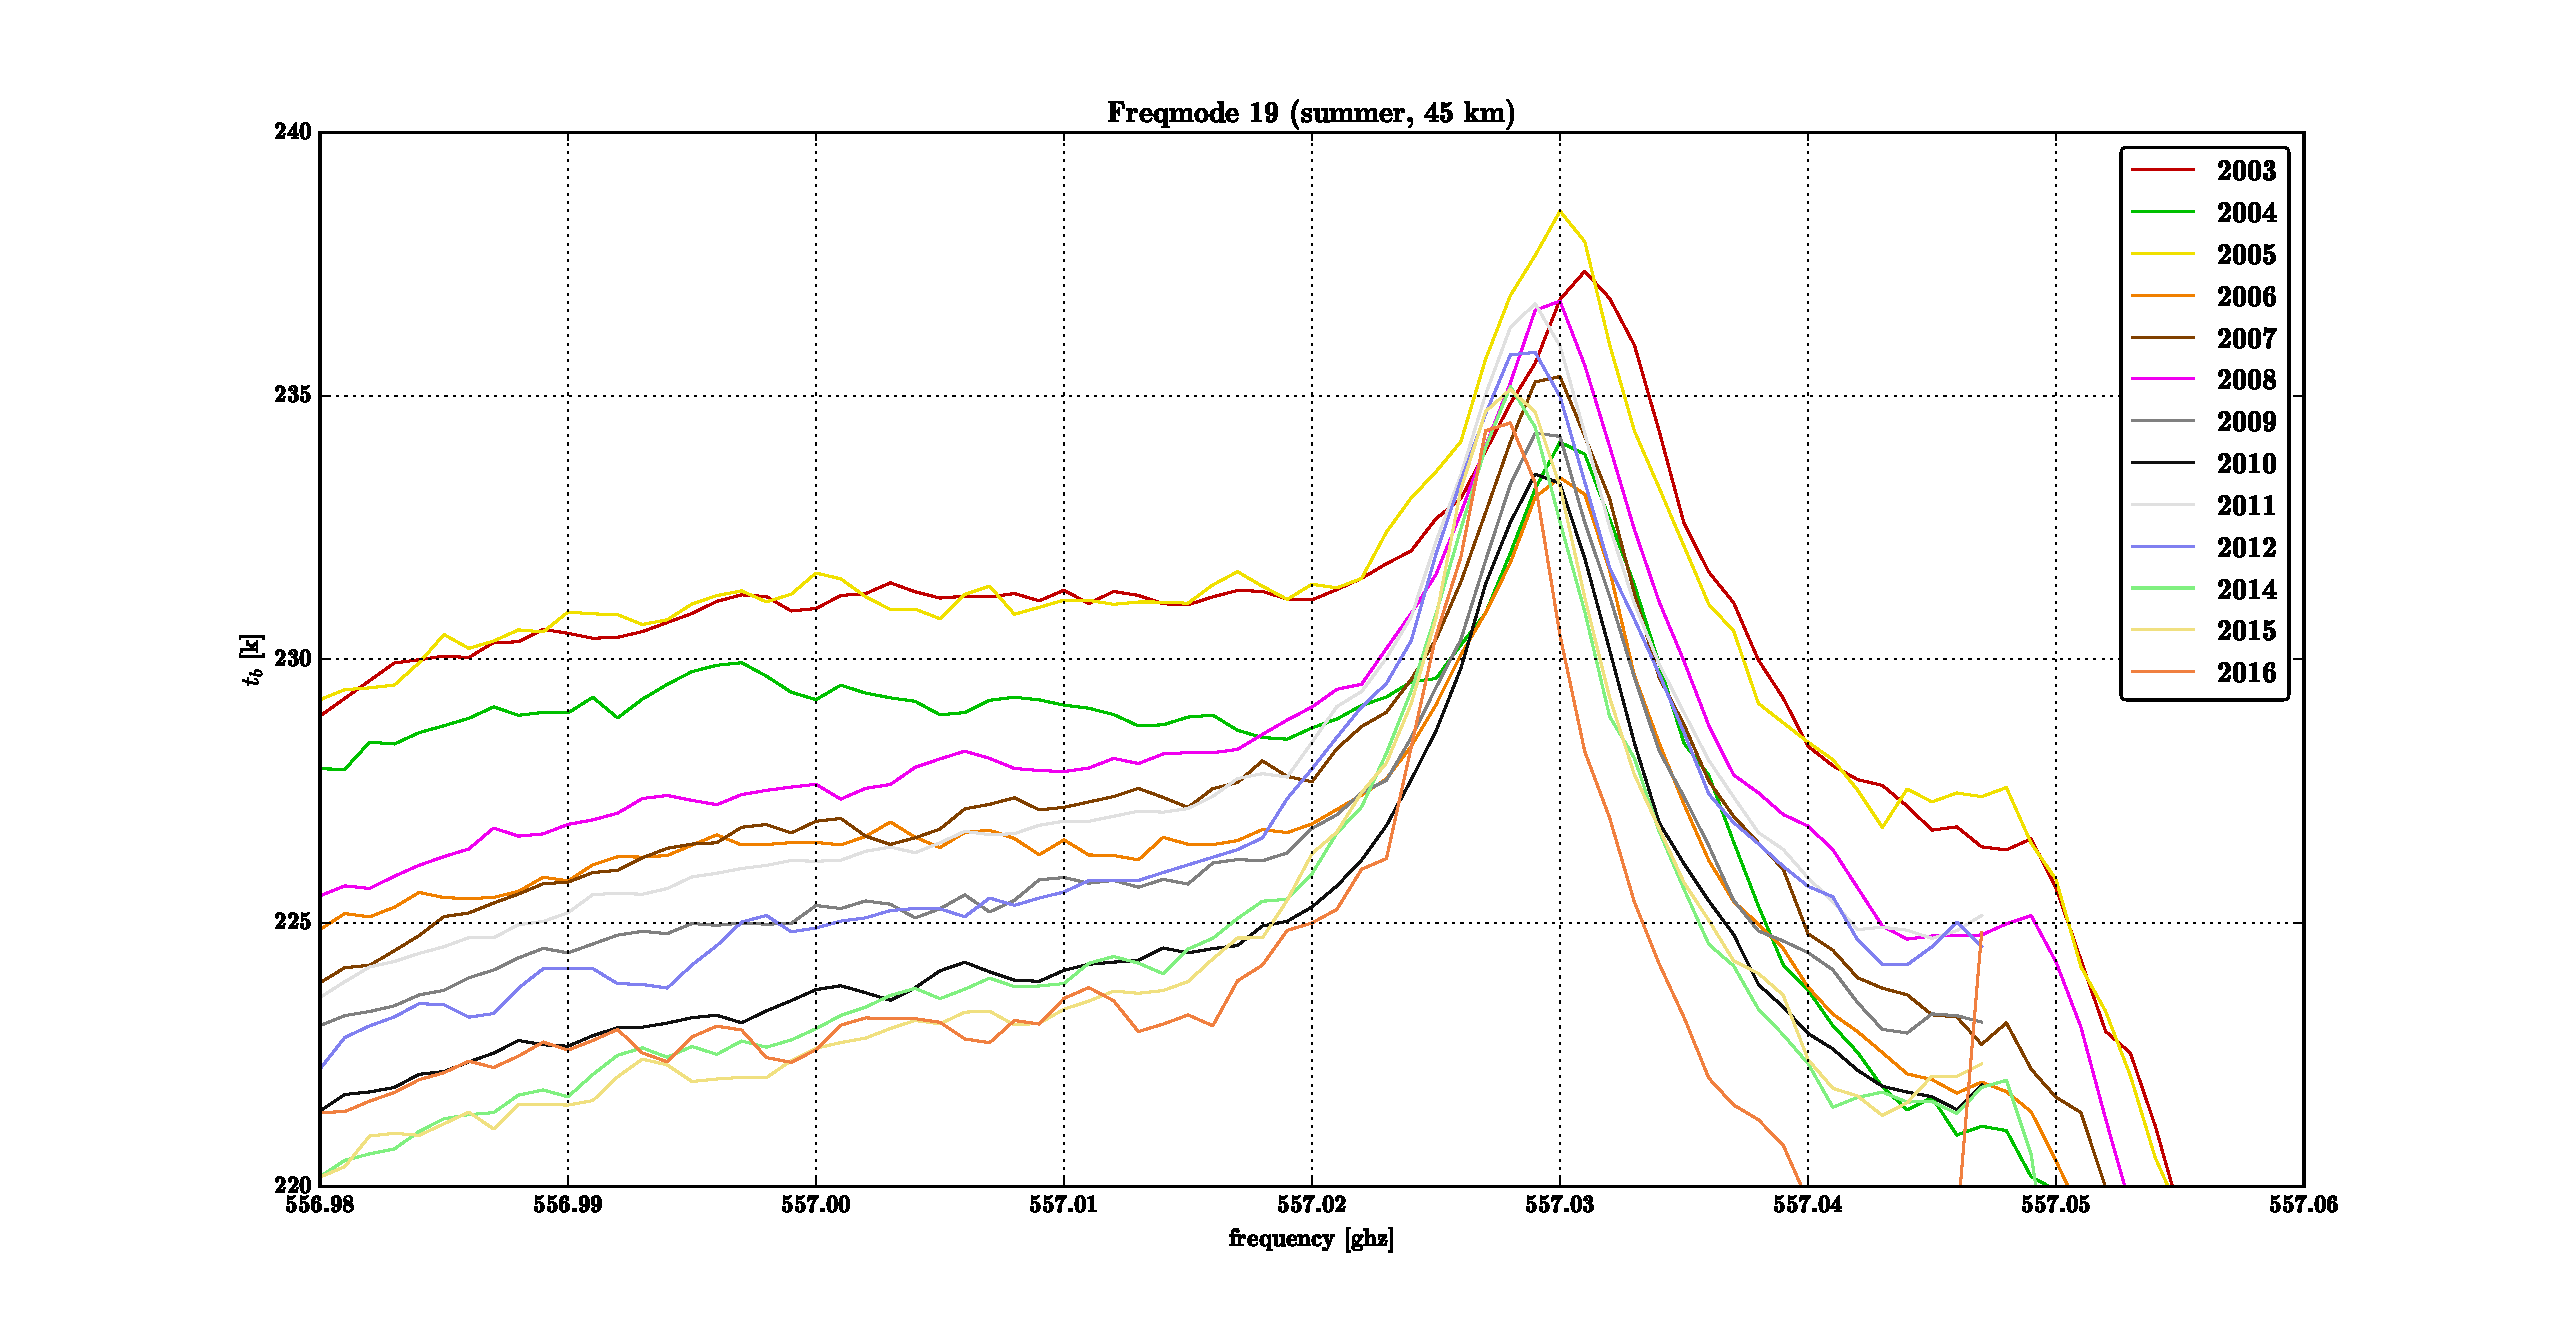
\includegraphics[width=\textwidth]{fm_19_spectra_summer_45km_sb}
        \caption{summer; 2014--2016 from FM~119
            }\label{fig:spectra:19:summer:closeup}
    \end{subfigure}
    \begin{subfigure}[b]{0.9545\textwidth}
        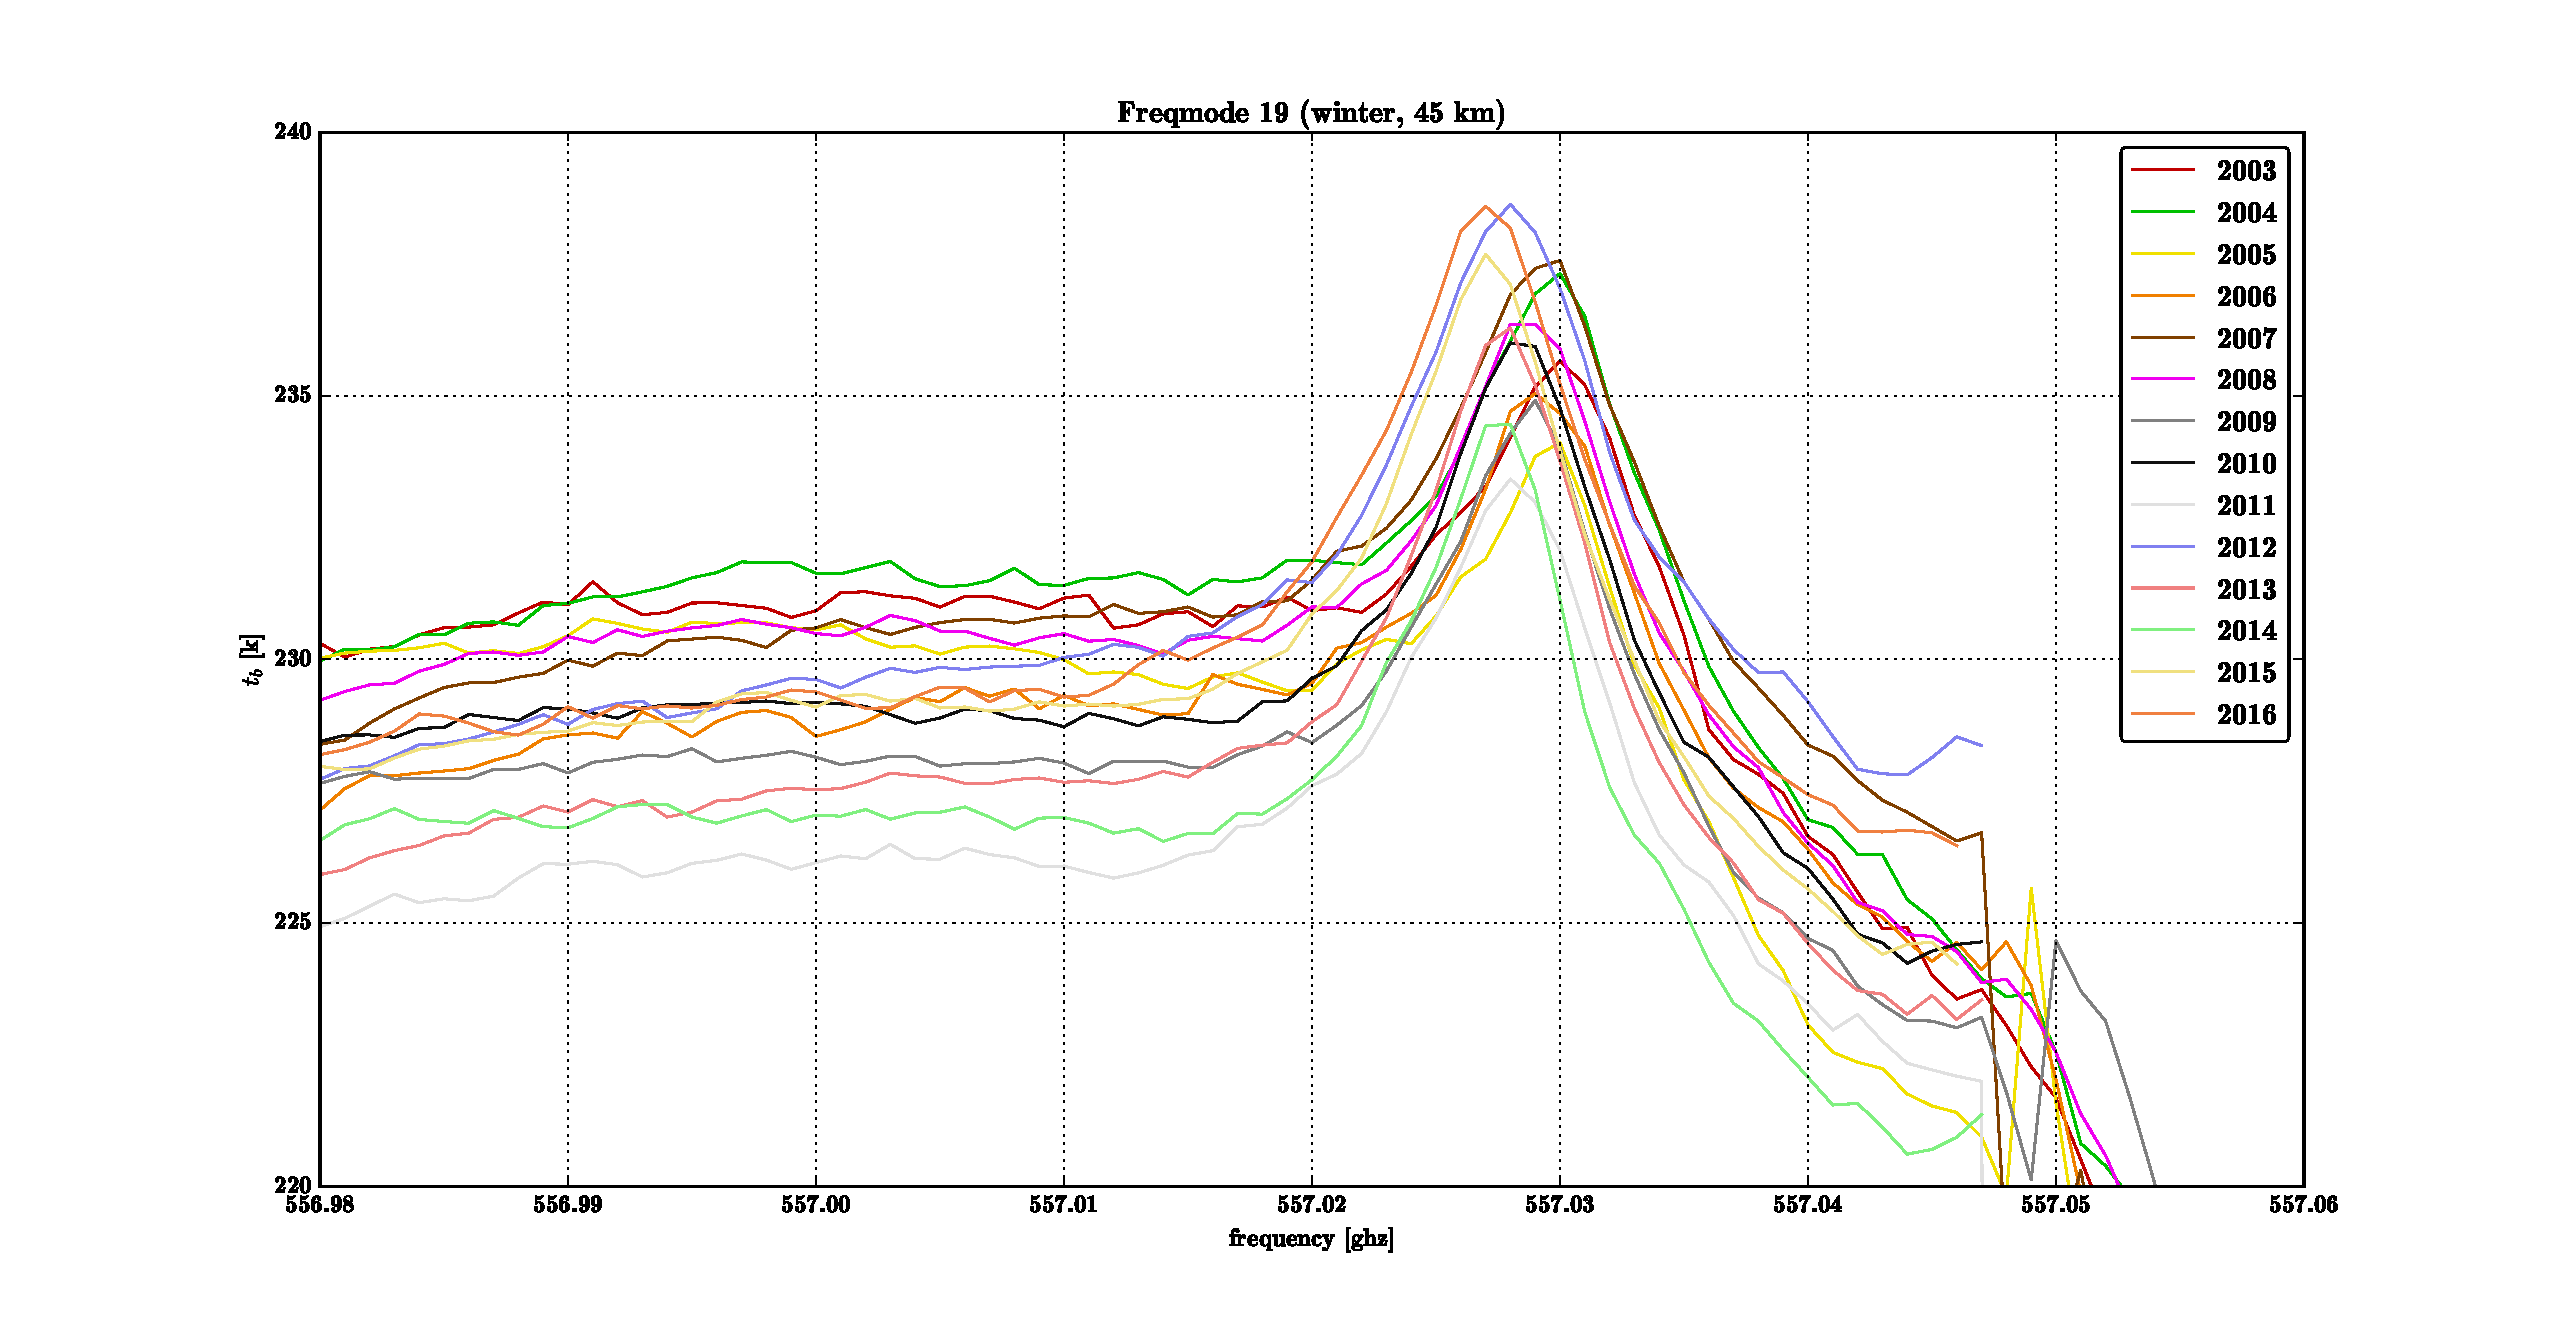
\includegraphics[width=\textwidth]{fm_19_spectra_winter_45km_sb}
        \caption{winter}\label{fig:spectra:19:winter:closeup}
    \end{subfigure}
    \caption{Close-up of right side of \chem{H_2O} peak and accompanying
        sideband \chem{O_3} peak in annual median spectra for FM~19
        for altitude interval 42--48~km at equatorial latitudes.  This area
        corresponds to that used to gauge the sideband leakage in
        Fig.~\ref{fig:sbl:19}.
        }\label{fig:spectra:19:closeup}
\end{figure}

\noindent
Yearly median spectra for summer and winter at $\sim45\,\mathrm{km}$ are shown
in Fig.~\ref{fig:spectra:19}.  These, and the close-ups of the right side the
water-vapour peak around $556.936\,\mathrm{GHz}$ seen in
Fig.~\ref{fig:spectra:19:closeup}, show that the peak appears to vary both in
height and width.  The tendency seems to be that the mainband peak is
decreasing, whereas the sideband peak is increasing.  This suggests the the
sideband leakage is increasing over time, which is investigated further in
Sec.~\ref{FM19:sbl}.


\subsection{Sideband leakage}
\label{FM19:sbl}

\begin{figure}[ht]
    \centering
    \begin{subfigure}[b]{0.9545\textwidth}
        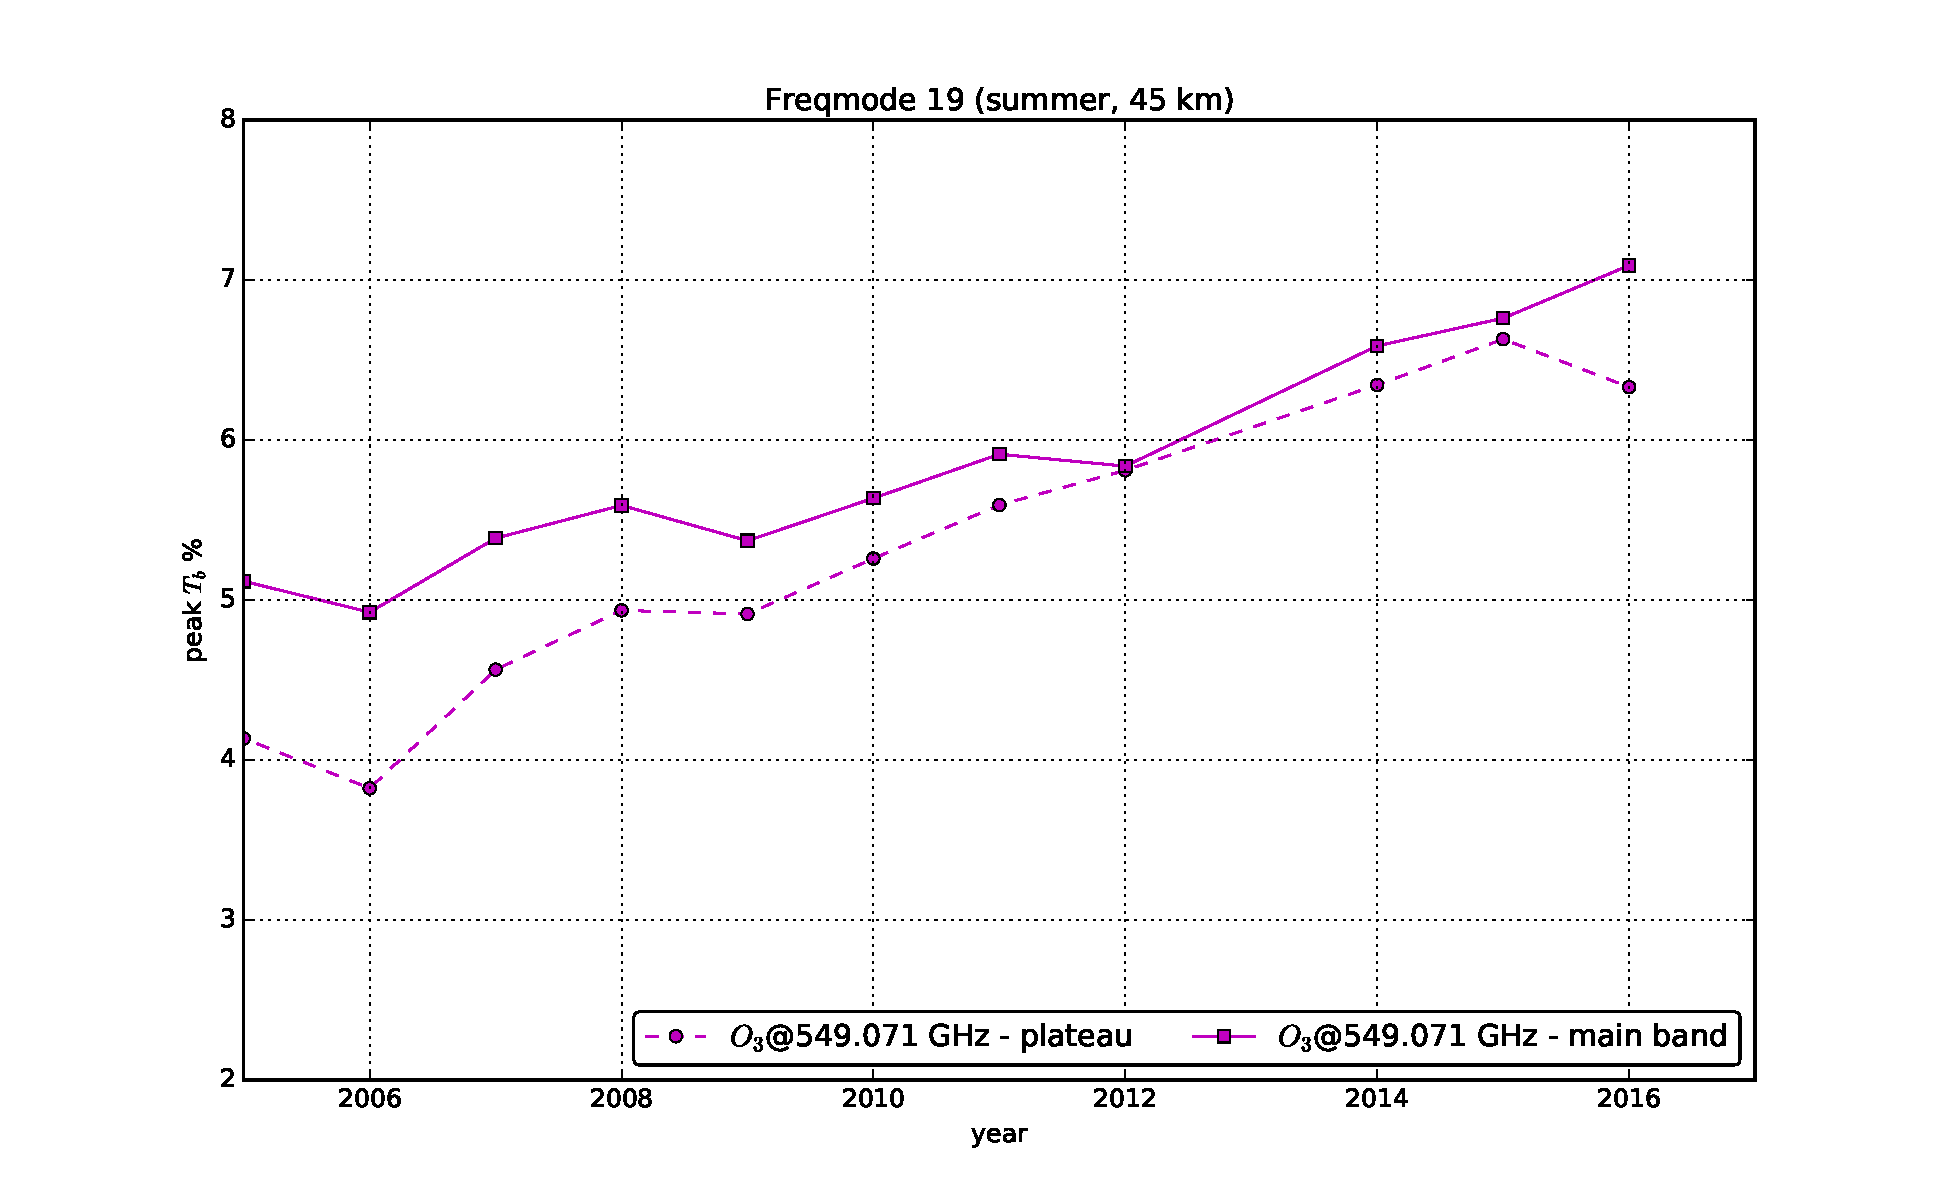
\includegraphics[width=\textwidth]{fm_19_peaks_summer_45km_sb_adjusted}
        \caption{summer; 2014--2016 from FM~119
            }\label{fig:sbl:19:summer}
    \end{subfigure}
    \begin{subfigure}[b]{0.9545\textwidth}
        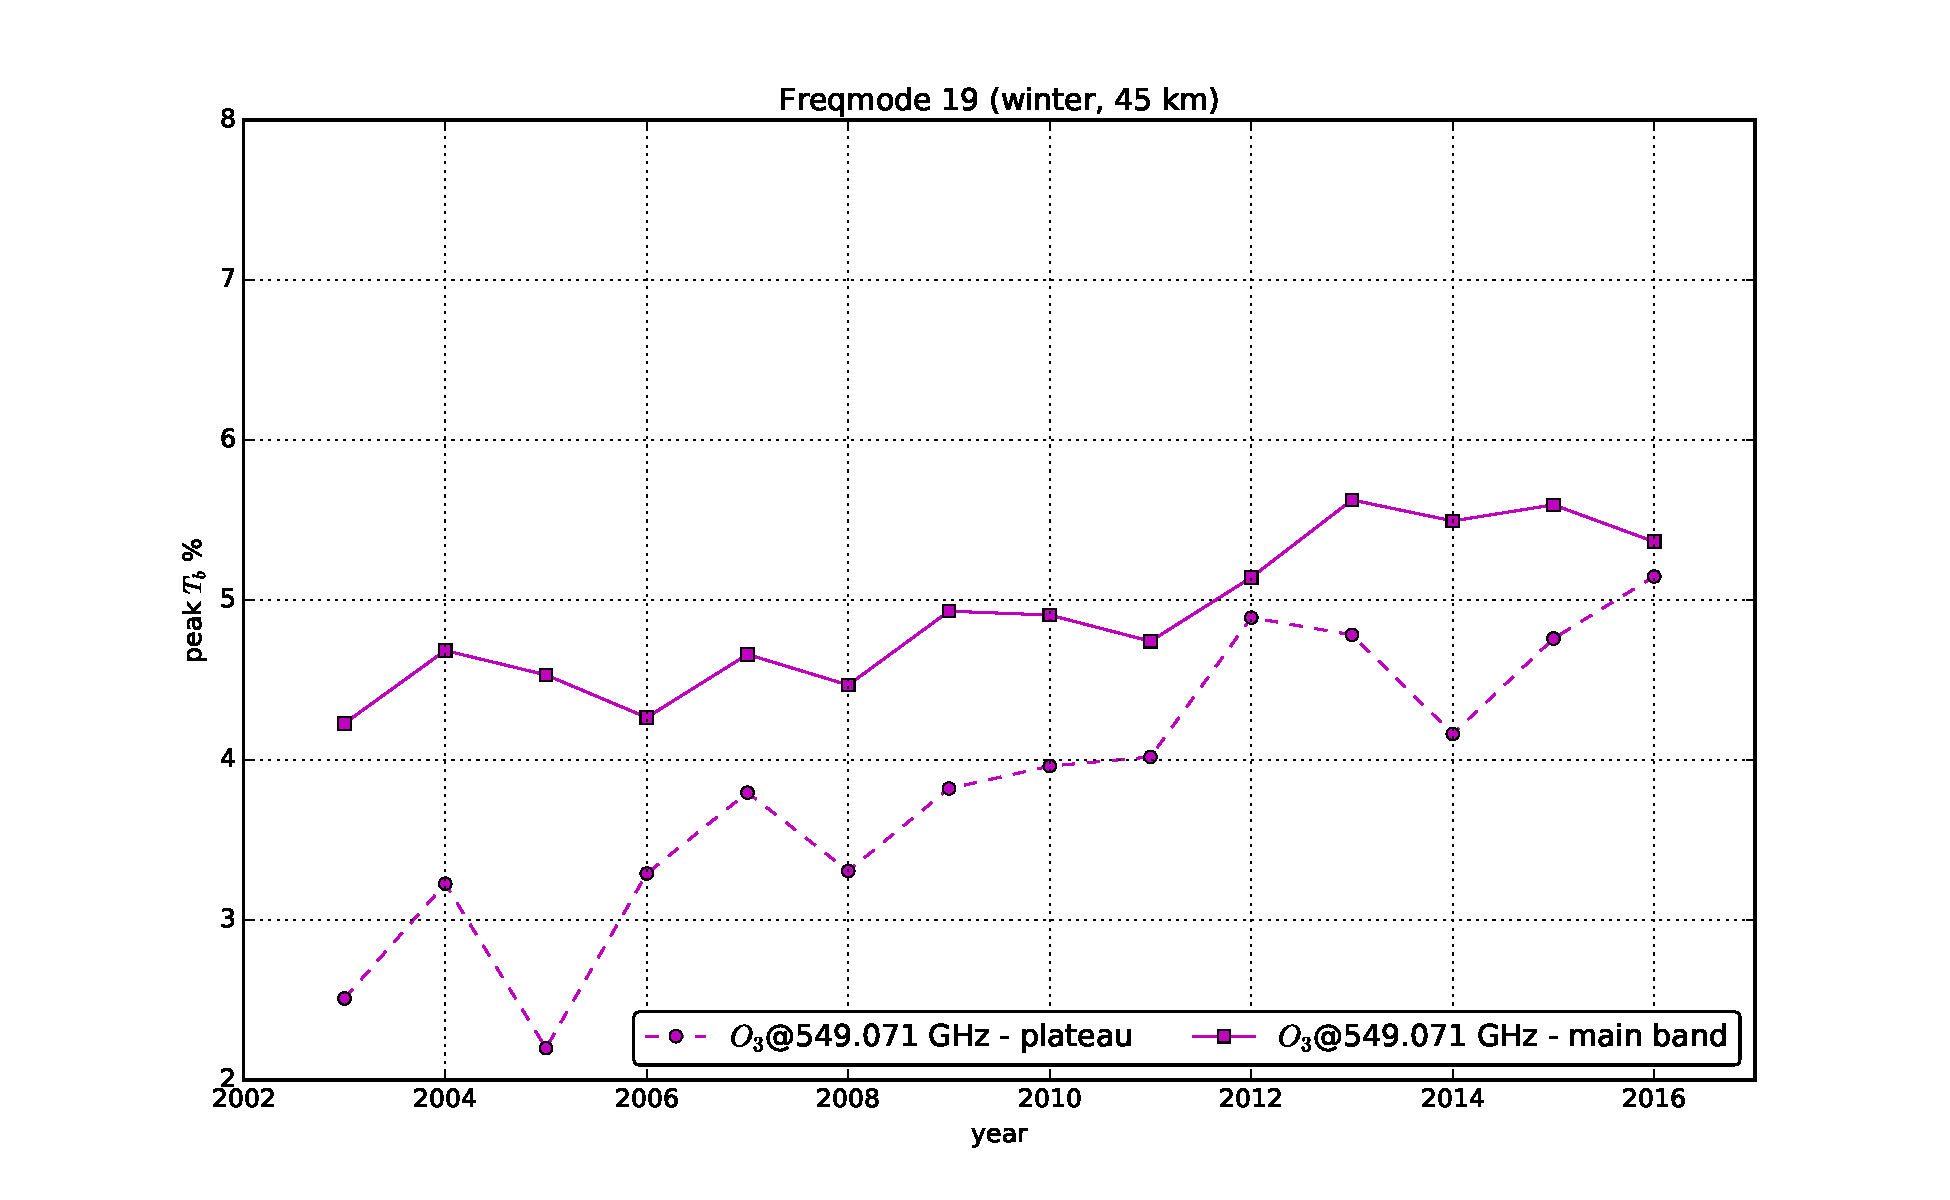
\includegraphics[width=\textwidth]{fm_19_peaks_winter_45km_sb_adjusted}
        \caption{winter}\label{fig:sbl:19:winter}
    \end{subfigure}
    \caption{Sideband leakage in \% calculated from the data shown in
        Fig.~\ref{fig:spectra:19:closeup}.  Values were calculated by
        subtracting the value of the plateau left of, or a first order
        approximation of the mainband value under, the peak.  The result was
        compared with $179.4\,\mathrm{K}$, a value deemed representative of the
        actual peak intensity.
        }\label{fig:sbl:19}
\end{figure}

\noindent
The sideband leakage was estimated at $\sim45\,\mathrm{km}$ by taking the
sideband peak intensity from the data shown in
Fig.~\ref{fig:spectra:19:closeup} and subtracing a the mainband intensity
estimated by two methods: by taking the value of the plateau to the left of the
peak, and by making first order approximation of the value directly under the
peak.  The actual value should between these two estimates, but closer to the
latter.  To estimate the leakage, the extracted peak intensities were then
divided by an expected sideband peak intensity from simulations
using ARTS~(\cite{buehler:artst:05}).  $179.4\,\mathrm{K}$ was chosen as a
representative, but the peak value varies by $\sim1\,\mathrm{K}$ from year to
year.  The results are shown in Fig.~\ref{fig:sbl:19} where it can be seen that
the sideband leakage appears to be increasing approximately linearly over time.
The sideband leakage also appears to be larger during the summer, when the
satellite is cold (see~Sec.~\ref{sec:Tcal}).  The tendency of the ``summer
mode'' FM~119 appears to be similar to that of FM~19, but with slightly
elevated values.  There is, however, too little data to draw any conclusions
regarding long term trends.


\subsubsection{Sideband paths}
\label{FM19:sbpath}
The sideband filter for FM~19 uses two more or less distinct values for the
sideband path length in equal measure: $-277.1\,\mathrm{\mu m}$ and
$-278.1\,\mu\mathrm{m}$.  The leakage tendency is the same for both categories,
and while a small difference in the level of leakage could ostensibly be seen,
it is much too small to recommend any change in settings.

The tendency of the ``summer mode'' FM~119 appears to be similar to that of
FM~19, though the difference in leakage between the two main paths is perhaps
more pronounced.  There is, however, too little data to draw any conclusions
regarding long term trends.

\subsection{Seasonality}
\label{FM19:seasonality}
The peak values of the \chem{H_2O} line at $\sim70\,\mathrm{km}$ during the
winter are consistently $\sim10\,\mathrm{K}$ higher than during the summer, as
can be seen in Fig.~\ref{fig:peaks:13v19}.  This could be due to natural
variations in the atmosphere or due to onboard conditions, such as increased
sideband leakage during the summer when the satellite is colder, as seen in
Fig.~\ref{fig:sbl:19}.


\subsection{Correlation with FM 13}
\label{FM19:FM13:corr}

\begin{figure}[ht]
    \centering
    \begin{subfigure}[b]{0.9545\textwidth}
        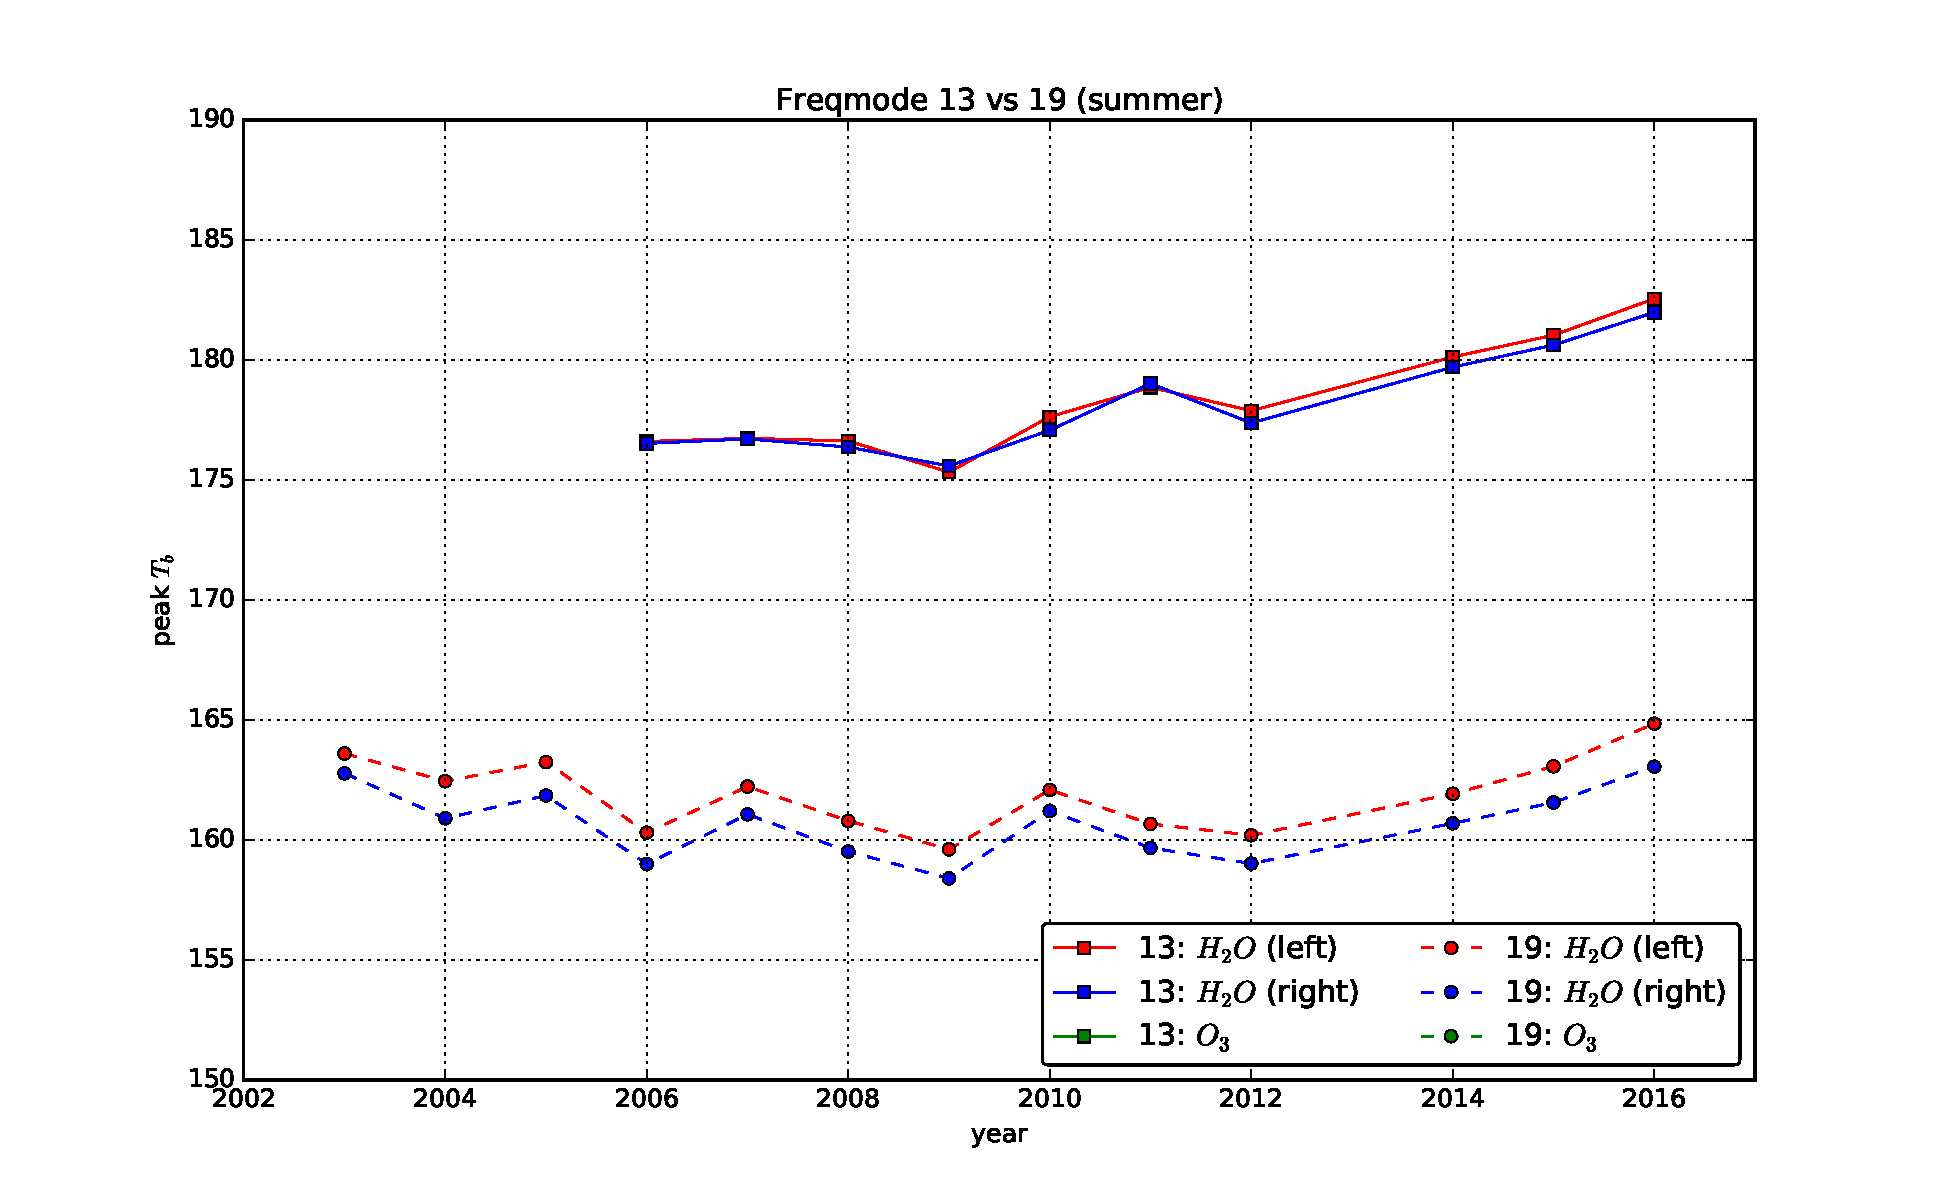
\includegraphics[width=\textwidth]{fm_13_vs_19_peaks_70km_summer}
        \caption{summer; 2014--2016 from FM~113 and~119.
            }\label{fig:peaks:13v19:summer}
    \end{subfigure}
    \begin{subfigure}[b]{0.9545\textwidth}
        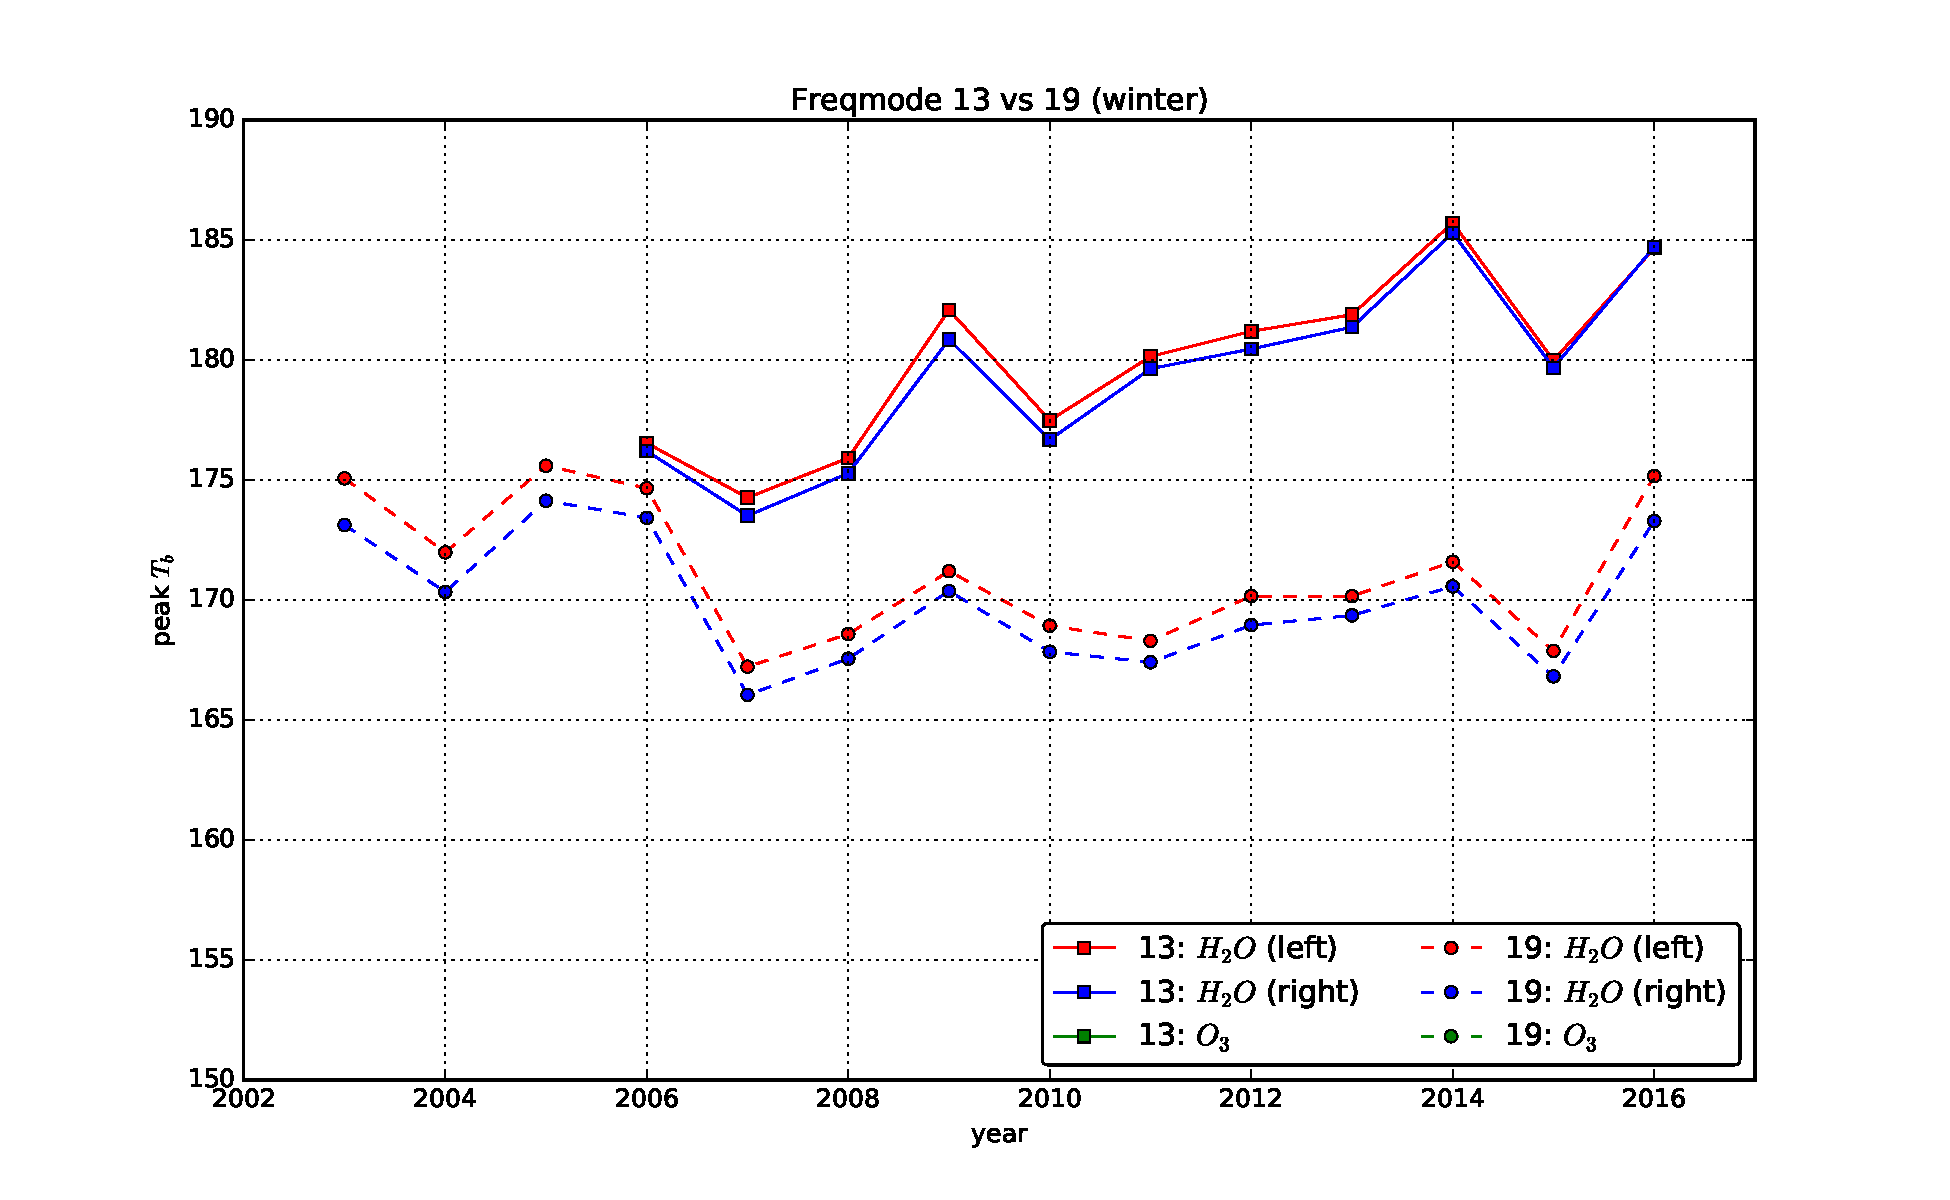
\includegraphics[width=\textwidth]{fm_13_vs_19_peaks_70km_winter}
        \caption{winter}\label{fig:peaks:13v19:winter}
    \end{subfigure}
    \caption{Peak values left and right of central dip in \chem{H_2O} peak in
        annual median spectra for FMs~13 and~19 for altitude interval
        65--75~km at equatorial latitudes.
    }\label{fig:peaks:13v19}
\end{figure}

\begin{figure}[ht]
    \centering
    \begin{subfigure}[b]{0.9545\textwidth}
        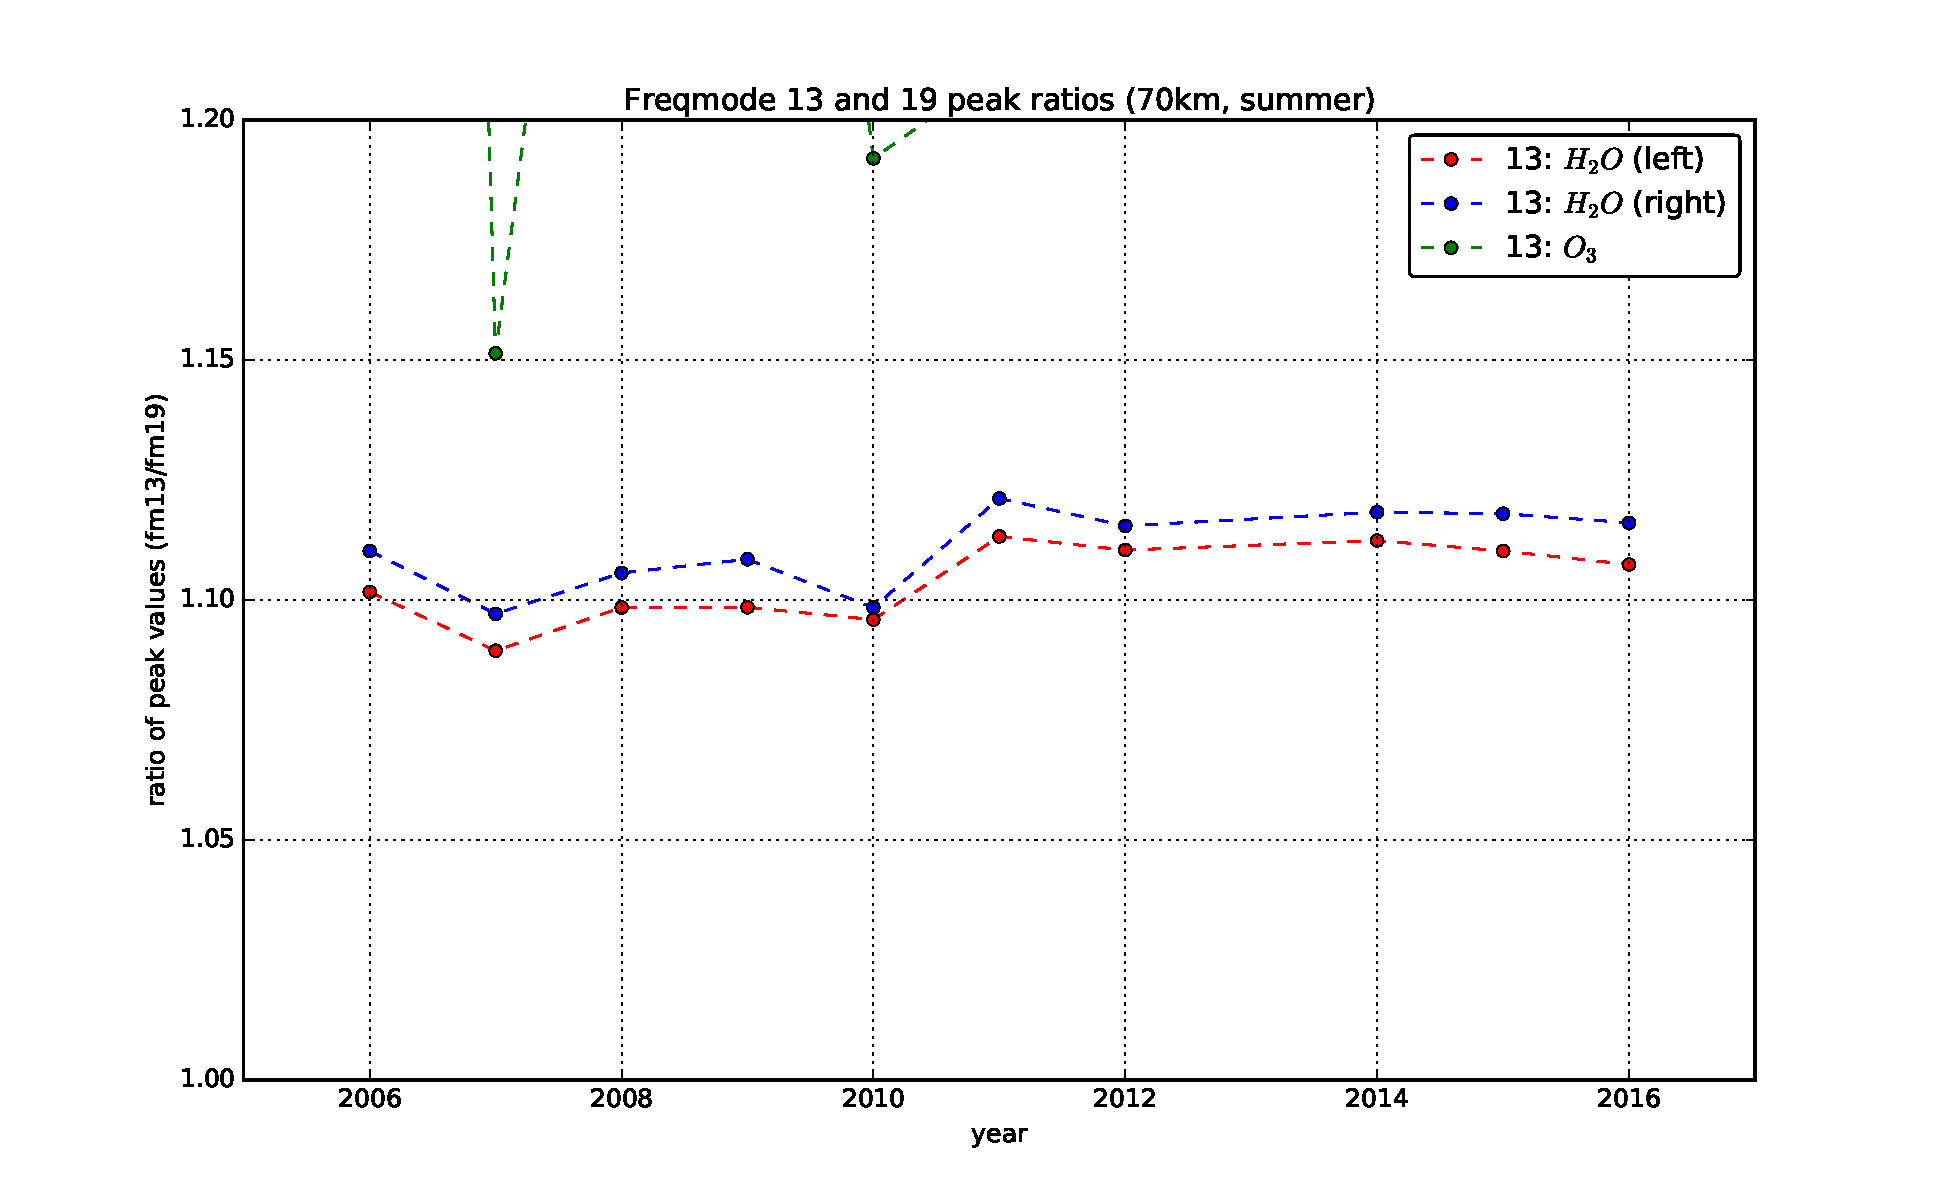
\includegraphics[width=\textwidth]{fm_13_vs_19_ratios_70km_summer}
        \caption{summer; 2014--2016 from FM~113 and~119.
            }\label{fig:ratios:13v19:summer}
    \end{subfigure}
    \begin{subfigure}[b]{0.9545\textwidth}
        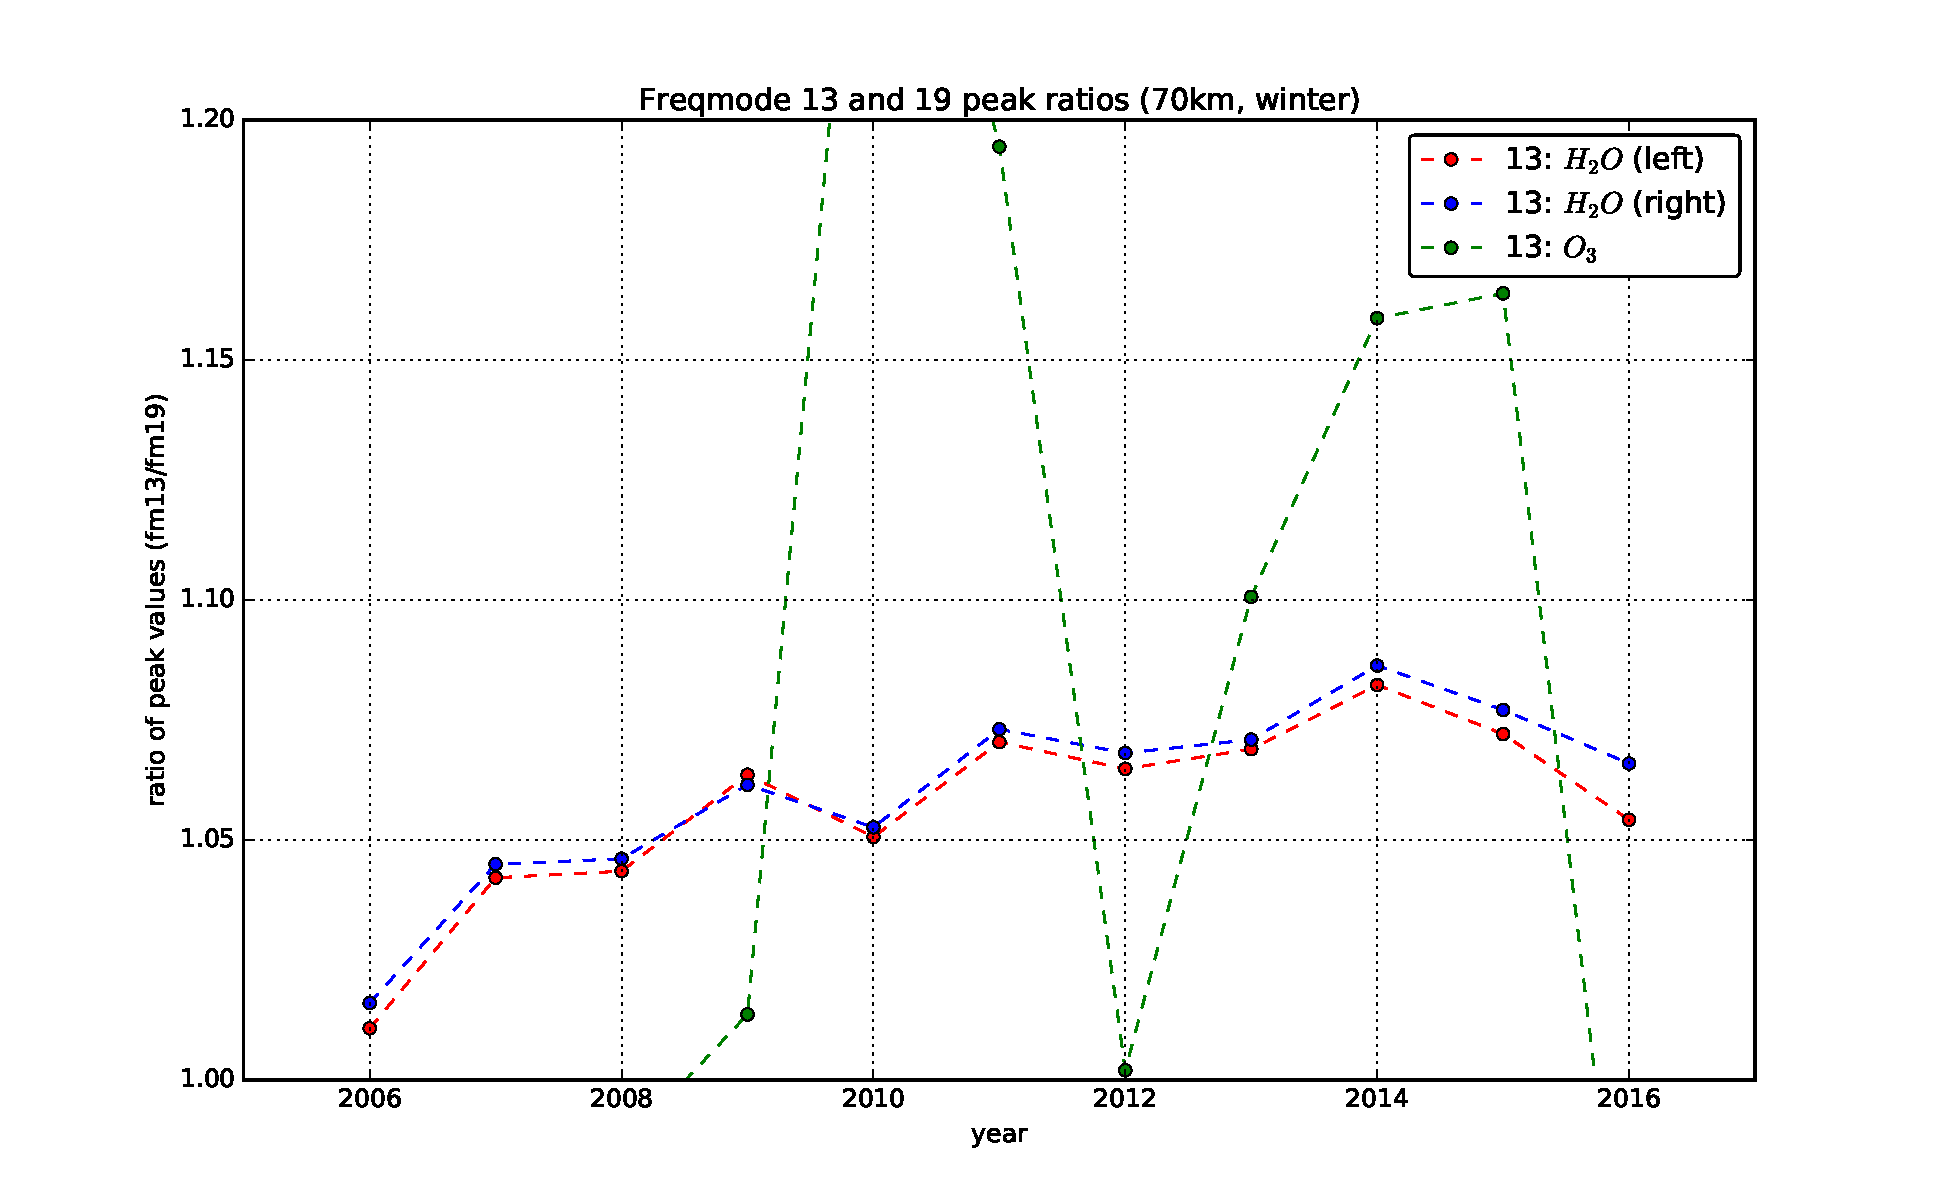
\includegraphics[width=\textwidth]{fm_13_vs_19_ratios_70km_winter}
        \caption{winter}\label{fig:ratios:13v19:winter}
    \end{subfigure}
    \caption{Ratios of FM~13 to FM~19 peak values left and right of central dip
        in \chem{H_2O} peak in annual median spectra for altitude interval
        65--75~km at equatorial latitudes.
    }\label{fig:ratios:13v19}
\end{figure}

\noindent
FM~19 was also investigated for the altitude interval 65--75~km with the
purpose to compare it with FM~13.  The spectra are qualitatively very similar to
those in Figs.~\ref{fig:spectra:13} and~\ref{fig:spectra:13:closeup} and are
therefore not shown here.  Instead we look at direct comparisons between FM~19
and FM~13.

As can be seen in Fig.~\ref{fig:peaks:13v19} FM~19 has a clear assymetry in the
that the left peak is consistently $\sim1\,\mathrm{K}$ lower than the right
peak, something which is not seen for FM~13.  It is also evident that FM~19
consistently underperforms compared to FM~13, both during summer and winter,
for the years when there is data for both modes.  As can be seen more clearly
in Fig.~\ref{fig:ratios:13v19}, the discrepancy is larger during the summer,
when the satellite is at its coldest.  It is interesting to note that during
the winters before 2007, when the satellite was warmer
(see~Sec.~\ref{sec:Tcal}), the FM~19 intensity was higher and also much closer
to that of FM~13.  The same trend is not seen during the summer, possibly
because the satellite was always colder then.  This suggest a higher
temperature sensistivity in FM~19 than in FM~13.

A further trend seen in Fig.~\ref{fig:peaks:13v19} is that the intensities
observed for FM~13 appear to be increasing with time after 2010.  This same
trend is not evident in the data for FM~19, at least not for the summers, as
can be seen from the ratios in Fig.~\ref{fig:ratios:13v19}.  The temperature on
the satellite for this period is relatively stable, except for seasonal
variations, wherefore this trend cannot be attributed to temperature
variations.

It is also noted here that the spectra from FM~19 and FM~119 do not exhibit the
same $1.5\,\mathrm{GHz}$ shift seen for FM~13 and FM~113 (see
Sec.~\ref{fig:spectra:13}).
